\documentclass[a4paper,12pt]{article}
\usepackage{graphicx}
\usepackage{hyperref}
\begin{document}
\title{Chomp
\subsubsection*{Requirements and Specification Document -- Group 6}\subsubsection*{Version 0.1}
}\maketitle

\renewcommand{\abstractname}{Project Abstract}
\begin{abstract}

Chomp is a web application that tracks what a person, group, or family eats, and gives nutritional advice, financial suggestions, sustainability ratings, and other meal and dietary statistical analysis.  Chomp provides a more digestable understanding of how our food affects us beyond a simple calorie counter.  By leveraging multiple informational APIs, a wealth of data can be generated from simple meal entries.  Customers use Chomp to gague their daily, weekly, monthly, and yearly progress toward their personal goals, and choose Chomp as their preffered tool because of its variety and wealth of information packed into a convenient and understandable form.  Plans for Chomp include adding a social support network of like-minded users to aid in users' feeling of and drive for success.  The anticipated revenue stream for Chomp will be in-app addvertisements that target a given user.

Our github location is \url{http://github.com/hedekar/chomp}
\end{abstract}
\newpage
\tableofcontents
\newpage
%%%%%%%%%%%%%%%%%%%%%%%%%%%%%%%%%%%%%%%%%%%%%%%%%%%
\section{Customers}
\subsection{Weight Loss}
This customer uses Chomp to keep a daily count of their calories and specific nutritional information to assist them in losing weight.  See \textbf{Appendix A.1} for the user persona of Boris Chetznekov for further info.
\subsection{Family Nutrition}
This customer uses Chomp to track how nutritious her family meals are and what deficiencies in the diet may need to be addressed.  She is also very concerned with meal cost.  See \textbf{Appendix A.2} for the user persona of Susan Montgomery for further info.
\subsection{Body Builder}
This customer uses Chomp to monitor his body's nutrition levels as he prepares for body building competitions.  He lives with two roommates who also work out, but not to the same level of competitiveness.  They all share groceries.  See \textbf{Appendix A.3} for the user persona of Chet Reist for further info.
%%%%%%%%%%%%%%%%%%%%%%%%%%%%%%%%%%%%%%%%%%%%%%%%%%%
\section{Competitive Analysis}
Many other meal-tracking services already exist.  Some have multiple million downloads and users.  The majority of these however are very specific in scope, with only calories being counted or with a focus on reporting all the nutritional numbers at once.  The large majority of these applications are targeting weight loss customers but not other users.\\
\\
Both web applications and mobile applications have been developed in this field.  Some specific competitors include: \begin{list}{•}{•}
\item \textbf{\href{http://www.noom.com}{Noom Coach -- noom.com} -- }A semi-free app that counts calories eaten and calories burned.  It then calculates and tracks weight of the user.  Includes 'coach' messages in a personalized manner.  The paid version allows for community sharing of progress and chatting amongst similar-goaled users as well as meal suggestions.  10-50million android downloads, 4.3 rating from 160,000+ reviews
\item \textbf{\href{http://www.myfitnesspal.com}{MyFitnessPal -- myfitnesspal.com} -- }
\item \textbf{\href{http://www.lifesum.com}{Lifesum -- lifesum.com}}
\item \textbf{\href{http://www.fatsecret.com}{FatSecret -- fatsecret.com}}
\item \textbf{\href{http://www.myfooddiary.com}{My Food Diary -- myfooddiary.com}}
\end{list}
%%%%%%%%%%%%%%%%%%%%%%%%%%%%%%%%%%%%%%%%%%%%%%%%%%%
\section{User Stories}
%%%%%%%%% to include in each story: Name/Description, Actors/Personas, Precondition/trigger, Actions/Post Condition, Acceptance Criteria, Tests
\subsection{User Accounts}
\textbf{Personas involved:} All\\
\textbf{Description:} These stories are all united under the epic of editing and using both new and existing user accounts.  New users must first complete the Registration story.  Returning users must first complete the Login story.  After these stories, users may then complete the Account Setup and Logout stories.
\subsubsection{Registration}
\textbf{Precondition:} An unrecognized or not-logged in user visits our frontpage.\\
\textbf{Actions:} A user is greeted with an interface requesting to register.  Options for both Google and Facebook account linkage (via their account APIs) will be presented as well as a manual entry field for e-mail and password. \begin{list}{•}{•}
\item Google's API registration will request the user for their google e-mail and password.  After this is submitted, the
\item Facebook's API registration will request the user for their Facebook e-mail and password.  This will then re-direct to a facebook window that asks the user to agree for us to get certain 
\item Manual entry process will request first name, last name, username, and e-mail.  This will be followed up by sending the user's e-mail a confirmation message in which a unique activation link will be sent.  The process will end at a page instructing users to look for their e-mail link that will allow them to finish setting up their account.
\end{list}
After registration completion, the system will send the user directly to the Account Setup stage.\\
\textbf{Test/Postcondition:} A new account should be attempted to be created via google, facebook, as well as manually and the database should register all of the user's submitted information.  To check, developers can access the database directly to see the adition.
\subsubsection{Account Setup}
\textbf{Precondition:} Either the user's account has freshly been registered, or they have clicked on the 'Account Settings' button of their user profile.\\
\textbf{Actions:} If the account is already setup, the dialogue will present the setup items as an editable listing rather than sequential prompts.  A dialogue will ask the user about the following items\begin{list}{•}{•}
\item Number of users to track (along with their usernames if they're also Chomp users)
\item Birthdate (of primary user and each non-Chomp user)
\item Current weight (of primary user and each non-Chomp user)
\item Height (of primary user and each non-Chomp user)
\item Personal priority ranking (eg. sustainability, carbohydrate intake, finances, etc..)
\end{list}
Once all of this information is submitted, the user's account will be updated and the desired statistics will take priority in the nutrition and value tracking interface.  The user will see the saved account settings filled out with the option to re-edit them or to return to the home screen.\\
\textbf{Test/Postcondition:} To confirm that the information was saved to the user's account the simplest method is to check the database entry manually.  Once the entire user interface has be implemented, the changes of this process should be visible immediately on the user's homescreen.
\subsubsection{Login}
\textbf{Precondition:} A registered user is returning to the site without a login cookie in their browser.\\
\textbf{Actions:} At the centre of the screen the both username or e-mail field and password field will display for the user.  Once the fields are filled out, the user clicks the Login button.  If any error occurs, the user is notified of the problem (in a semi-specific manner that helps users without assisting intrusion attempts).  If no error occurs the user is taken to their Chomp homepage.\\
If an unregistered username or e-mail is entered, the registration process should begin for the user with a notice that the e-mail does not seem to be registered yet.\\
\textbf{Test/Postcondition:} An unregistered e-mail should be tried, at which time the user should be led to the registration story.  A registered account should be entered, first with an incorrect password, at which time an error message should appear, and then with a correct password, at which time the homescreen should appear.
\subsubsection{Logout}
\textbf{Precondition:} A user must be logged into their account.\\
\textbf{Actions:} By hovering over the user's name in the top-right corner of the screen a drop down menu will appear that includes the logout button.  The user then clicks this button and is greeted with the login screen.\\
\textbf{Test/Postcondition:} Follow the logout steps.  The login page should be reached.  Then attempt to visit a particular page of the user's profile.  This test should return an error.
%%%%%%%%%%%%%%%%%%%%%%%%%%%%%%%%%%%%%%%%%%%%%%%%%%%
\section{User Interface Requirements}
There are three major sections of our user interface that should be considered critical to the application's success.  Furthermore, we have ideas for expansion and additional feature that we will describe briefly in this section.
\subsection{Critical Interfaces}
\subsubsection{Meal Entry Dialogue}
This dialogue should allow entry for time of meal, contents of meal, and portion of meal.  Eventually, the ability to edit previous meals will also be added.
\subsubsection{Personal Nutrient \& Value Tracking}
This section of the homepage should give weekly, monthly, and yearly charts of the user's desired reporting figures and any additional abnormal trends our algorithm notices.
\subsubsection{Account Goal and Preference Adjustment}
This section is the user's administrative section over their entire account.  Here they can tweak what they want Chomp to help them with.
\subsection{Additional Interface Ideas}
\subsubsection{Suggested Meal Listing}
\subsubsection{Community Support Feed}
\subsubsection{Grocery Bill/List Tracking}
%%%%%%%%%%%%%%%%%%%%%%%%%%%%%%%%%%%%%%%%%%%%%%%%%%%
\newpage 
\appendix
\section{User Personas}
\subsection{Boris Chetznekov}

\includegraphics[scale=0.3]{Boris.jpg}\\
\textbf{Age:} 58\\
\textbf{Weight:} 370lbs\\
\textbf{Occupation:} Office Manager for the city's traffic department\\
\textbf{}
\textbf{Goal: }To not die early.  After years of gross caloric intake his doctor has informed him of his impending death if his diet and weight doesn't change immediately.\\
\begin{large}
\textbf{\textit{"I guess I have to change my ways; stupid doctors.  Hopefully I can still drink a beer or vodka or two."}}
\end{large}

\subsection{Susan Montgomery}

\includegraphics[scale=0.23]{Susan.jpg}\\
\textbf{Age:} 33\\
\textbf{Weight:} 143lbs\\
\subsection{Chet Reist}
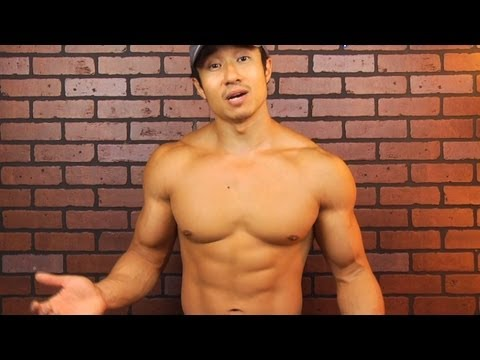
\includegraphics[scale=0.38]{Chet.jpg}\\
\textbf{Age:} 21\\
\textbf{Weight:} 170lbs\\
\end{document}